\documentclass[aspectratio=169]{beamer}
\usepackage{pgf}

\mode<presentation>
{
%   \usetheme{Madrid}
%   \useinnertheme{circles}
  \setbeamertemplate{navigation symbols}{}
%   \usetheme[hideothersubsections, width=2.4cm]{Hannover}
%   \usetheme{Antibes}
%   \usetheme{Montpellier}
  \usetheme{Singapore}
%   \usecolortheme{seahorse}
   \setbeamertemplate{footline}
   {%
%      \begin{beamercolorbox}{section in head/foot}
%       \usebeamercolor{bg}
       \hskip 1em \footnotesize \insertframenumber{} / \inserttotalframenumber%\hskip 41em \includegraphics[height = .5cm]{../../../../bilder/cc_by-nc_eu.png}
% % cc_by-nc_eu.png: 403x141 px, 72dpi, 14.22x4.97 cm, bb=0 0 403 141
%
% % bwslogo_3.png: 476x392 px, 300dpi, 4.03x3.32 cm, bb=0 0 114 94
%
%       %\hskip 5em
%       %       \input{../bilder/cc_by.png}
%       %\includegraphics[height=.5cm]{../../../../bilder/bwslogo_3.png}
%      \end{beamercolorbox}%
   }
  \usepackage{beamerfoils}
}

\usepackage[german]{babel}
\usepackage[utf8]{inputenc}
\usepackage{times}
\usepackage[T1]{fontenc}
\usepackage{eurosym}
\usepackage{graphicx}
\usepackage{amsmath}
\usepackage[siunitx,european]{circuitikz}
\usepackage{ulem}
\usepackage{listings}
%
\lstset{numbers=left, numberstyle=\tiny, stepnumber=2, numbersep=5pt, language = C++, captionpos=b, alsolanguage=XML, basicstyle=\ttfamily}
% \MyLogo{\includegraphics[height=1cm]{../../../../bilder/bwslogo_3.png}}
% % \includegraphics{../../bilder/bwslogo_3.png}
% % bwslogo_3.png: 476x392 px, 300dpi, 4.03x3.32 cm, bb=
%


\only<presentation>{
  \usepackage{hyperref}
}


\title{Arbeitsunterlagen zu Prin im BG Praktische Informatik}

\date{V 0.1.0 - im Aufbau\\ Stand: \today}%\\

\institute[BWS Hofheim]{Brühlwiesenschule, Hofheim}
\author{Thomas Maul}

\titlegraphic{Für eigene Teile gilt: \includegraphics[height=1cm]{cc_by-nc_eu.png}}

\begin{document}
% \begin{frame}<beamer>
%   \titlepage
%   % \hyperlink{Teil_2}{\beamerbutton{Go part 2}}
% \end{frame}
% \AtBeginSection[] % Do nothing for \section*
% {
%   \begin{frame}<beamer>
%     \frametitle{Inhalt}
%     \tableofcontents[currentsection]
%   \end{frame}
% }



\section{Objektreferenz}

\begin{frame}{Objektreferenz}
 \begin{itemize}
  \item Ein Array mit Pointern (als Attribut der Klasse)
  \item Verweis auf Objekte (auf dem Heap)
  \item Umsortieren ist einfach, da nur Pointer kopiert werden.
 \end{itemize}
\end{frame}

\begin{frame}[fragile]
  \frametitle{Klasse DataModel}
  \begin{lstlisting}
  class DataModel
{
public:
    DataModel();
    static const unsigned short arraySizeEntry = 20;
    void insertEntry(int pos, int val);
    void removeEntry(int pos);
    int findEntryPos(int pos);
    int findEntryVal(int val);
    bool appendEntryBack(int val);

private:
    Entry* entryAray[arraySizeEntry];///< Links auf die Objekte
                                     // in der Warteschlange.
};
 \end{lstlisting}
\end{frame}

\section{Ring-Puffer}
\begin{frame}{Ring-Puffer}
 \begin{itemize}
  \item Array ist linear.
  \item Problem: Kontinuierliche Messwerte, \\
  alte werden automatich überschrieben.
  \item logisch: Ring
  \item zwei ``Zeiger'' (schreiben / lesen)
  \pause
  \item reale Struktur: Array (in der Regel)
 \end{itemize}
\end{frame} 

\begin{frame}{Realisierung}
 \begin{itemize}
  \item Array für Werte (z.B. Array für Int)
  \item Zeiger lesen und Zeiger schreiben
  \item Lesen darf schreiben nicht überholen
  \item Wenn schreiben am Ende des Arrays ist, \\
  Sprung auf Pos 0. Ggf. Lese-Zeiger verschieben.
 \end{itemize}
\end{frame}

\begin{frame}{Visualisierung}
 \begin{figure}
 \centering
 \only<1>{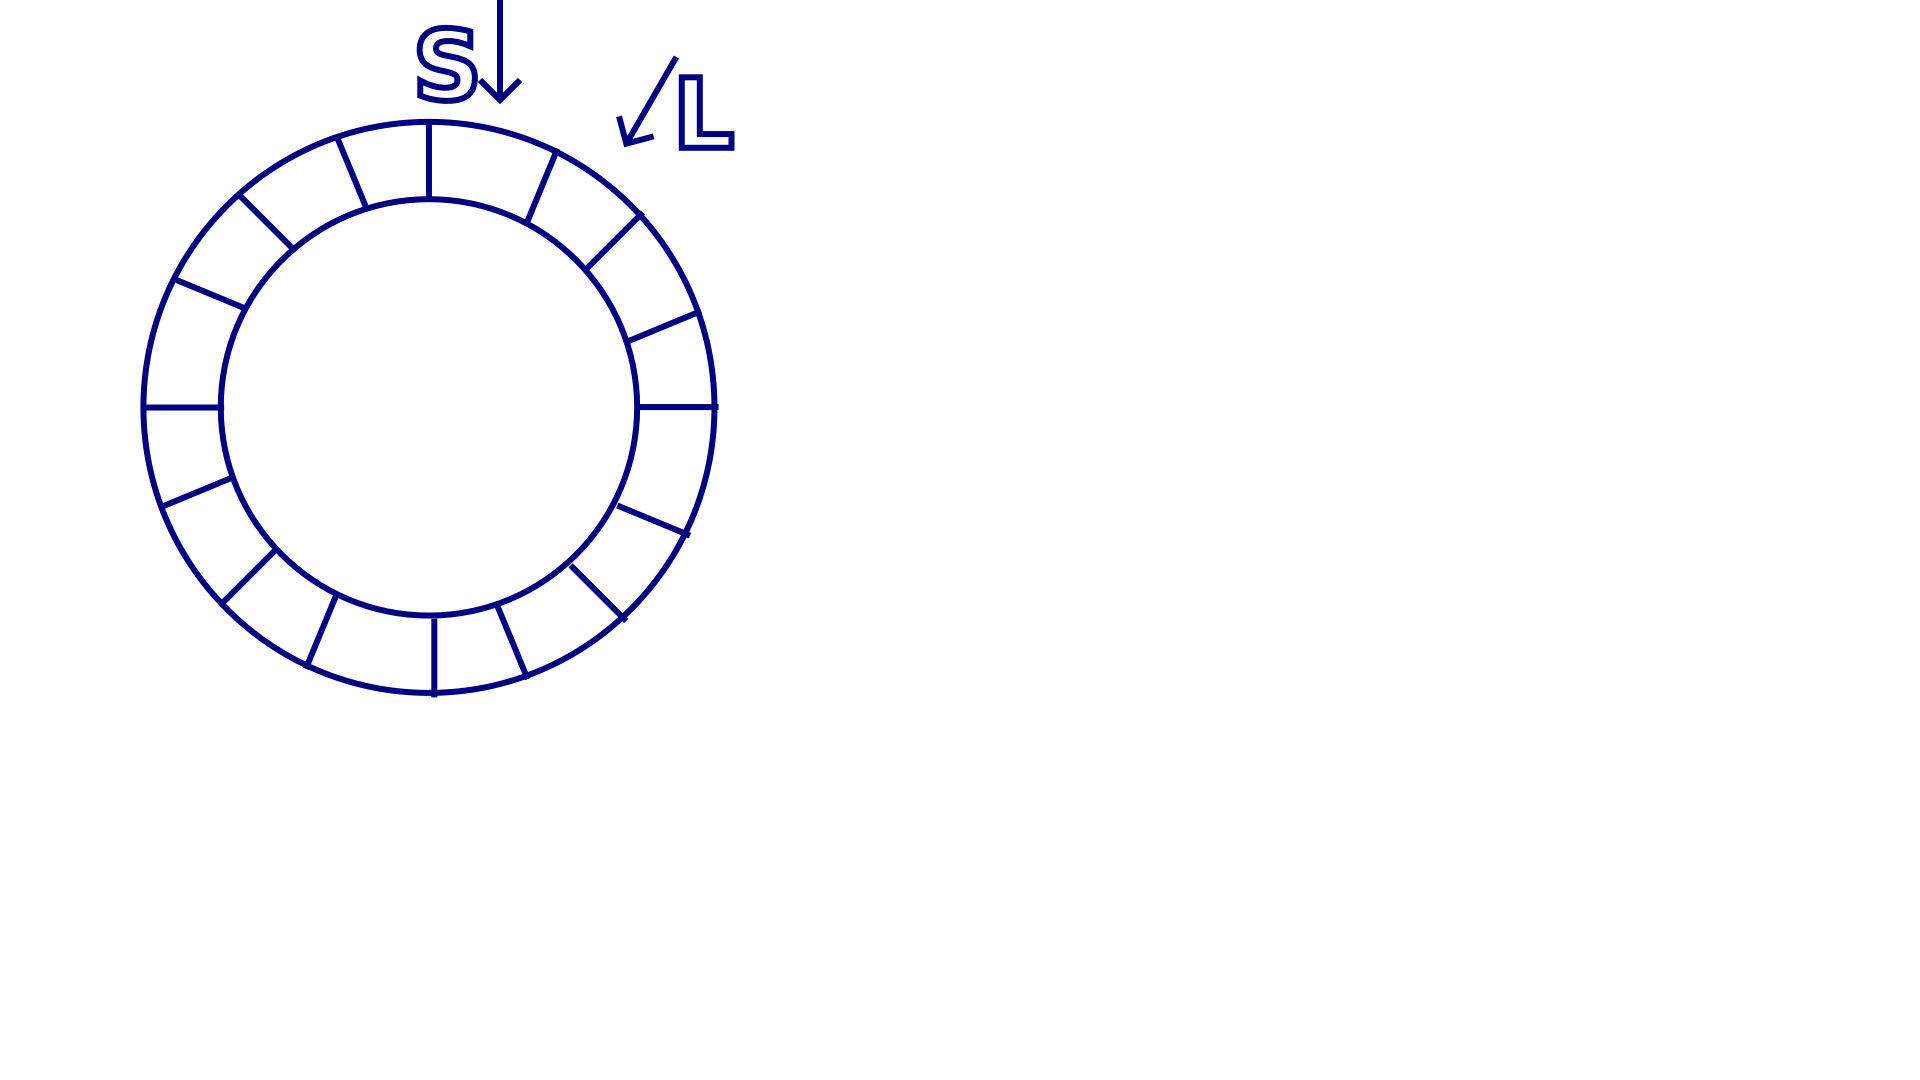
\includegraphics[height=.9\textheight]{ringpuffer1.png}
 % ringpuffer1.png: 0x0 px, 0dpi, nanxnan cm, bb=
 \label{abb:Ringpuffer1}}

 \only<2>{\includegraphics[height=.9\textheight]{ringpuffer2.png}
 % ringpuffer1.png: 0x0 px, 0dpi, nanxnan cm, bb=
 \label{abb:Ringpuffer2}}
 
 \only<3>{\includegraphics[height=.9\textheight]{ringpuffer3.png}
 % ringpuffer1.png: 0x0 px, 0dpi, nanxnan cm, bb=
 \label{abb:Ringpuffer3}}
 
 \only<4>{\includegraphics[height=.9\textheight]{ringpuffer4.png}
 % ringpuffer1.png: 0x0 px, 0dpi, nanxnan cm, bb=
 \label{abb:Ringpuffer4}}
 
 \only<5>{\includegraphics[height=.9\textheight]{ringpuffer5.png}
 % ringpuffer1.png: 0x0 px, 0dpi, nanxnan cm, bb=
 \label{abb:Ringpuffer5}}
 
 \only<6>{\includegraphics[height=.9\textheight]{ringpuffer6.png}
 % ringpuffer1.png: 0x0 px, 0dpi, nanxnan cm, bb=
 \label{abb:Ringpuffe6}}

 \only<7>{\includegraphics[height=.9\textheight]{ringpuffer7.png}
 % ringpuffer1.png: 0x0 px, 0dpi, nanxnan cm, bb=
 \label{abb:Ringpuffe7}}
\end{figure}

 
\end{frame}




  \label{LastPage}
\end{document}
